% El objetivo de esta parte será aprender a utilizar referencias, tanto para elementos del documento como ecuaciones o secciones, como para referencias externas (bibliografía).

% Un aditivo importante para esta parte es el archivo .bib que se encuentra en la carpeta. Lo veremos cuando sea el momento.

\documentclass{article}

% Paquetes %
\usepackage[utf8]{inputenc} 
\usepackage[spanish]{babel}
\usepackage{mathtools, amsfonts, amsmath, amsthm, amssymb}
\usepackage{setspace}
\usepackage{graphics}

% El siguiente paquete nos permite un manejo más fino de la posición de las imágenes y tablas.
\usepackage{float} 

% Márgenes y espaciado %
\usepackage[margin=2cm]{geometry}
\spacing{1.2}

% Para usar bibliografía usaremos un paquete especial. Lo hacemos porque es moderno y nos permite ordenarnos mejor, pero no es estrictamente necesario. El paquete se llama biblatex. Además, podemos determinar el estilo y ordenamiento de nuestra bibliografía usando opciones:
%	-	La opción style define el estilo de escritura de la referencia. Aquí usaremos numeric, pero pueden ver otros estilos aquí: https://www.overleaf.com/learn/latex/Biblatex_bibliography_styles. En particular, la opción draft permite ver las abreviaciones que pusimos en el archivo bib y puede ser útil para llevar un seguimiento de estas.
%	-	La opción sorting dice cómo se ordena la bibliografía. Aquí usaremos ynt que significa que las referencias se ordenan por año-nombre del autor-título (year-name-title). Pueden encontrar otras formas de ordenamiento aquí: https://www.overleaf.com/learn/latex/Bibliography_management_with_biblatex#Reference_guide.
%	- 	La opción citestyle determina cómo aparece la cita en el texto. Aquí usaremos authoryear, que escribe el autor y el año.
%	-	La opción backend es más técnica y dejaremos el valor recomendado que es biber.
%	-	Finalmente, la opción natbib nos permite usar otros comandos de cita para que se vea más bonito.
\usepackage[style = numeric,
			sorting = ynt,
			citestyle = authoryear,
			backend = biber,
			natbib]{biblatex}

% Le debemos decir a biblatex de dónde obtendrá las referencias. En nuestro caso están en el archivo bib que se llama references y para incorporarlo usaremos el comando \addbibresource:
\addbibresource{references.bib}

% Ahora es un buen momento para revisar ese archivo.

% Para cerrar la introducción bibliográfica, notar que para compilar un documento con bibliografía el proceso es ligeramente más tedioso si no se ocupa Overleaf o similares. En el caso que estemos trabajando con un editor que no compila la bibliografía automáticamente, debemos hacer el siguiente proceso:
%	Compilar LaTeX --> Compilar BibTeX/Biber --> Volver a compilar LaTeX

% Este procedimiento debe hacerse cada vez que se incorpora una cita nueva. Si solo incorporamos texto entonces no es necesario.

% ADVERTENCIA IMPORTANTE SI NO USAN OVERLEAF: Muchos editores NO tienen a biber seleccionado de manera predeterminada para manejar bibliografía. Si este ejemplo no funciona para ti, revisa cómo seleccionar biber mirando esta página: https://tex.stackexchange.com/questions/154751/biblatex-with-biber-configuring-my-editor-to-avoid-undefined-citations/439854#439854

% Antes de empezar miraremos dos paquetes importantes para referencias.

% El primero, hyperref, permite crear múltiples links a objetos dentro y fuera del texto. Pero más aún se encarga de manejar la estética de estos links. En este caso cargaremos el paquete con la opción colorlinks para que todas las referencias aparezcan en colores y pondremos esos colores en azul con la opción allcolors. Se puede personalizar que cosas diferentes tengan colores distintos, pero por ahora esto bastará.
\usepackage[colorlinks, allcolors=blue]{hyperref}

% El segundo es cleveref, hace que las referencias dentro del texto a imagenes y otros objetos sean más fáciles de crear y más claras. A nosotros nos interesa un comando en particular que discutiremos luego.
\usepackage[spanish]{cleveref}

% Lamentablemente, el paquete cleveref tiene pésimos nombres para algunos de los elementos (apartado en lugar de sección o cuadro en lugar de tabla). Para cambiar estos nombres manualmente usamos el comando \crefname. La sintaxis es:
%		\crefname{objeto}{nombreSingular}{nombrePlural}

% Debemos cuidar de poner el segundo y tercer argumentos en minúsculas.
\crefname{section}{sección}{secciones}
\crefname{table}{tabla}{tablas}

% Es importante notar que para que la referencia aparezca correctamente en el texto, se debe compilar LaTeX dos veces.

% Documento %
\begin{document}

\section{Introducción}

En este ejemplo revisaremos cómo se utilizan referencias en un documento de {\LaTeX}. Para ello cargamos muchos algunos paquetes en el preámbulo y algunas citas desde el journal QJE. En particular tenemos las citas de \citet{policeViolence}, \citet{religionAndEconomy} y \citet{crimesMorality}. Estas referencias se obtuvieron escribiendo \texttt{\textbackslash citet\{abreviacion\}}, con la abreviación que utilizamos en el archivo \texttt{bib}.	\\

Pero también podemos hacer referencias a otras partes del documento como secciones, subsecciones, imágenes, tablas e incluso ecuaciones. Para hacerlo la norma es seguir dos pasos: 1) crear un nombre para el lugar u objeto que se quiere referenciar y 2) llamar a esa referencia en algún lugar del texto.	\\

Para lo primero, se debe crear un \texttt{label} para el elemento deseado con el comando \texttt{\textbackslash label\{nombreDelLabel\}}. El \texttt{nombreDelLabel} debe ser distintivo para que nosotros mismos seamos capaces de entender qué estamos citando. Por ejemplo, si queremos referenciar una sección que se llame ``Mi Seccion'', un nombre para su label podría ser \texttt{sec:MiSeccion}. Con \texttt{sec} dejamos claro que es una sección y los ``\texttt{:}'' nos sirven para que la lectura del label sea más claro. Algunos editores además guardan los labels por nosotros en una lista que podemos revisar. Es importante saber que el comando \texttt{\textbackslash label} se ubica dentro del entorno correspondiente si es una imagen, tabla o ecuación; y justo después de la definición de la sección o la subsección, si es el caso.	\\

Una vez creado el label, debemos decirle a {\LaTeX} que incluya la referencia en una parte del texto. Para este ejemplo, hemos puesto un label para cada una de las secciones del texto, las cuales referenciaremos con el comando \texttt{\textbackslash Cref{nombreDelLabel}} Por ejemplo, el label \texttt{sec:RefImagenes} sirve para referenciar a la \Cref{sec:RefImagenes}. Podemos referenciar varios elementos a la vez, separando labels con ``,'' en el comando \texttt{\textbackslash Cref}. Por ejemplo, las \Cref{sec:RefTablas,sec:RefEcuaciones,sec:RefURLs} nos ayudaran a referencias tablas, ecuaciones y URLs, respectivamente.

\section{Referenciando imágenes} \label{sec:RefImagenes}

Muchas veces nuestros documentos incluirán imágenes con gráficos o diagramas asociados a nuestro trabajo. Referenciarlas es muy fácil y la sintaxis que aprenderemos en esta sección aplicará también a las tablas y a las ecuaciones. Recordar la dupla \texttt{label}-\texttt{Cref} para referenciar.\\

Partiremos incluyendo la imagen justo aquí. Para referenciar correctamente la imagen la incluiremos dentro de un entorno llamado \texttt{figure}. En este entorno incluiremos el comando \texttt{includegraphics}, el \texttt{label} y un título para la imagen con el comando \texttt{caption}.

\begin{figure}[H] % Con la opción ``H'' le decimos a LaTeX que ubique la imagen justo aquí. De lo contrario, LaTeX elige la mejor parte del texto dónde ubicarla (que puede ser muy lejos de este lugar)

	% Al igual que las tablas, las imágenes no están centradas por defecto. Para centrarlas usaremos el comando \centering que funciona dentro de los entornos figure y table (este último lo veremos en la siguiente sección). 
	\centering

	% El título de la imagen va con el comando \caption
	\caption{Aquí va el título de la figura.}
	
	% Y ahora pondremos el label. Notar que usamos fig como prefijo para que recordemos que esta referencia corresponde a una imagen.
	\label{fig:patito}
	
	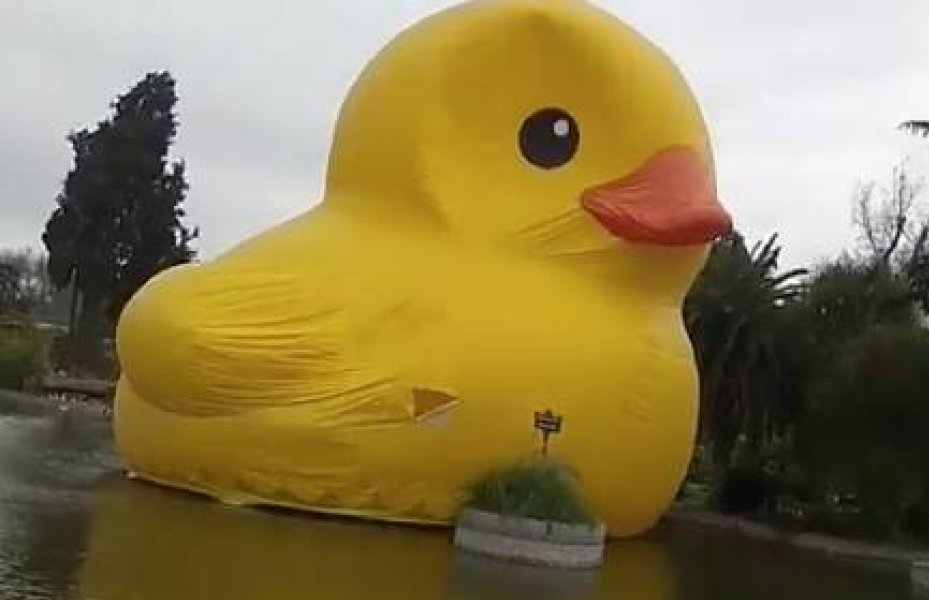
\includegraphics[width=0.5\textwidth]{pobrepatito} % Con la opción width definida de esta manera la imagen tiene un ancho igual a la mitad del ancho del texto.
\end{figure}

Ahora para referenciar la imagen seguimos la misma sintaxis que como lo hicimos par las secciones. Si lo recuerdan, el inflable que se ve en la \Cref{fig:patito} fue ubicado en una laguna de Santiago y sufrió un accidente, por lo que se desinfló.\\

Vale recordar que no importa si \texttt{label} va antes que \texttt{Cref}. Esto es claro si recordamos que referenciamos las secciones posteriores durante la introducción.

\section{Referenciando tablas} \label{sec:RefTablas}	

Las tablas son probablemente infaltables en un trabajo académico. Referenciarlas sigue la misma lógica que para las imágenes, pero en lugar de usar el entorno \texttt{figure} usamos el entorno \texttt{table}. Para fortalecer la idea que no es necesario tener \texttt{label} antes de \texttt{Cref}, estudiaremos la \Cref{tab:contenidos} a continuación.\\

Este curso basó su introducción en 5 pilares principales: crear documentos, escribir textos, incorporar imágenes y portadas, crear funciones y entornos y elementos numerados. En el último pilar se incluyen crear secciones, tablas, arrays, matrices y listas. Los contenidos de cada sección principal están indicados en la tercera columna de la \Cref{tab:contenidos}. 

\begin{table}[H]
	\centering
	\caption{Tabla de contenidos del curso de \LaTeX.}
	\label{tab:contenidos}
	
	\begin{tabular}{c | c | c}
		Tutorial	&	Título								&	Contenidos	\\ \hline
		1		&	Creación de documentos					&	Clases de documentos, paquetes, escritura de texto simple	\\ \hline
		2		&	Escritura de un texto simple				&	Márgenes, entornos, escritura de un texto complejo				\\ \hline
		3		&	Incorporar imágenes y una portada			&	Incorporación de portadas, manejo de imágenes	\\ \hline
		4		&	Crear funciones y un nuevo entorno			&	Creación de funciones y entornos con numeración heredada	\\ \hline
		5		&	Secciones, tablas, arrays, matrices y listas	&	Uso de tablas y arrays, escritura de matrices y uso de listas
	\end{tabular}
\end{table}

\section{Referenciando ecuaciones} \label{sec:RefEcuaciones}

Las ecuaciones matemáticas son un ingrediente muy común en el trabajo de un economista. Ya sean especificaciones econométricas o ecuaciones de un modelo teórico, sin duda tendrán que usarlas. Para referenciarlas, necesitamos que la ecuación esté dentro del entorno \texttt{equation} y dentro de ese entorno ponemos el \texttt{label}. En este caso, la \cref{eq:obviedad} muestra una de las operaciones matemáticas clásicas:
	\begin{equation} \label{eq:obviedad}
		1 + 1 = 2 
	\end{equation}

También es posible referenciar una o varias ecuaciones dentro de un entorno \texttt{align}. Por ejemplo, en las \cref{eq:cantidades,eq:precios} se presentan las condiciones que determinan un equilibrio de un mercado en competencia perfecta:
	\begin{align}
		Q_{d}	&=	Q_{s}	\label{eq:cantidades}\\
		P_{d}	&=	P_{s}	\label{eq:precios}
	\end{align}

En particular, la \cref{eq:cantidades} dice que la cantidad demandada y ofrecida deben ser iguales, mientras que la \cref{eq:precios} dice que los precios percibidos por demandantes y oferentes también deben ser los mismos.

\section{Bonus track: URLs} \label{sec:RefURLs}

A pesar de que no es demasiado común, hay veces donde queremos mostrar links a páginas web, por ejemplo, a una noticia o un hilo de Twitter. Para hacer esto usaremos el comando \texttt{href}. La sintaxis de este comando es \texttt{\textbackslash href\{URL\}\{nombre que aparece en el texto\}}. También se puede escribir sin el segundo argumento pero eso dificulta la lectura, dado que toda la dirección de la página aparecerá en el texto. Por ejemplo, \href{https://github.com/pipeton8/latex-course}{este link} dirige a la página de GitHub que contiene a este curso.\\

En este siguiente ejemplo, presionando en \href{https://twitter.com/dog_rates/status/1295801698221346816?s=20}{este link} podrán ver un lindo video de un perrito.

\printbibliography

\end{document}

